\chapter{Addytywna synteza dźwięku}\label{chapter_additive}
Synteza addytywna pozwala na utworzenie barwy dźwięku poprzez zbudowanie pełnego widma częstotliwościowego za pomocą odpowiednich składowych. Słowo 'addytywna' odnosi się do sumowania wielu przebiegów w jeden złożony sygnał dźwiękowy. Historycznie jest ona drugą najstarszą metodą syntezy, zaraz po subtraktywnej, opisanej w rozdziale \ref{chapter_subtractive}.
Zazwyczaj synteza addytywna polega na dodawaniu wielu fal sinusoidalnych o różnych częstotliwościach oraz amplitudach. Metoda ta pozwala jednak na dużą dowolność. Dodawanymi składowywmi sygnału nie muszą być jedynie fale sinusoidalne.
Synteza addytywna uznawana jest za odwrotność syntezy subtraktywnej. Znajduje zastosowanie w syntezie dźwięku oraz mowy.

W niniejszym rozdziale przedstawiono zasadę działania syntezy addytywnej. Zaprezentowano wzory matematyczne, za pomocą których można uzyskać zsyntezowane brzmienie. Przedstawiono również kilka metod implementacji tego rodzaju syntezy. Na końcu rozdziału zaprezentowano autorski interfejs użytkownika oraz wyniki zaimplementowania syntezy addytywnej na procesorze DSP.

\section{Zasada działania syntezy addytywnej}
Synteza addytywna jest zbliżona pod niektórymi względami do analizy częstotliwościowej Fouriera. Z tego powodu jest ona zaliczana do widmowych metod syntezy. Jej postać matematyczną można jednak przedstawić również w dziedzinie czasu. Zależnie od doboru składowych dźwięku, postać syntezy addytywnej może mieć różne reprezentacje \cite{add_defins}.
% Okresowosc sygnalu y(t)
%https://ccrma.stanford.edu/~jos/sasp/Additive_Synthesis_Early_Sinusoidal.html

\subsection{Postać harmoniczna} \label{pos_harm}
Dźwięk powstały w wyniku użycia syntezy addytywnej w formie harmonicznej można zapisać w postaci:
%https://en.wikipedia.org/wiki/Additive_synthesis#:~:text=Additive%20synthesis%20is%20a%20sound,or%20inharmonic%20partials%20or%20overtones.
\begin{equation} \label{equ:addit_time_harm}
y(t) = \sum_{k=1}^{K} a_{k}sin(2\pi kf_{0}t + \phi_{k})  \\  
\end{equation}
\begin{tabular}{ l l l l}
	gdzie: & $y(t)$ &  - & wyjście addytywnej syntezy dźwięku, \\
	&	$k$ & - &  numer składowej harmonicznej sygnału, \\
	&	$K$ & - &  całkowita liczba składowych harmonicznych dźwięku,\\
	&	$f_{0}$ & - &  częstotliwość pierwszej składowej harmonicznej,\\
	&	$a_{k}$ & - &  amplituda składowej harmonicznej k, \\
	&	$\phi_{k}$ & - &  faza składowej harmonicznej k. \\
\end{tabular} \\

Każda składowa dźwięku uzyskanego z takiej postaci syntezy addytywnej jest wielokrotnością częstototliwości podstawowej $f_{0}$. Wykorzystanie takiej postaci pozwala na utworzenie dźwięku na przykład organów. Jest to najbardziej podstawowy rodzaj syntezy addytywnej.

%https://en.wikibooks.org/wiki/Sound_Synthesis_Theory/Additive_Synthesis <<---- SCHEMAT 

%https://en.wikipedia.org/wiki/Square_wave
\begin{equation} \label{equ:addit_sqr}
y_{Square}(t) = \sum_{k=1}^{K} \frac{1}{2k-1} sin(2\pi (2k-1)f_{0}t) \\
\end{equation}

%https://en.wikipedia.org/wiki/Triangle_wave
\begin{equation} \label{equ:addit_trng}
y_{Triangle}(t) = \sum_{k=1}^{K} \frac{(-1)^k}{(2k-1)^2} sin(2\pi (2k-1)f_{0}t)  \\
\end{equation}

%https://en.wikipedia.org/wiki/Sawtooth_wave
\begin{equation} \label{equ:addit_sawth}
y_{Sawtooth}(t) = \sum_{k=1}^{K} \frac{(-1)^k}{k} sin(2\pi kf_{0}t) \\
\end{equation}
% O tym że na tym polegały organy Hammonda

Postać harmoniczna syntezy addytywnej pozwala również na uzyskanie podstawowych przebiegów używanych w syntezie subtraktywnej. Każdy z nich można wygenerować za pomocą sumowania odpowiednich składowych harmonicznych z odpowiednimi amplitudami. Przykłady takich przebiegów w formie ciągłoczasowej przedstawiono we wzorach (\ref{equ:addit_sqr}), (\ref{equ:addit_trng}) oraz (\ref{equ:addit_sawth}).

\begin{figure}[H]
	\centering
	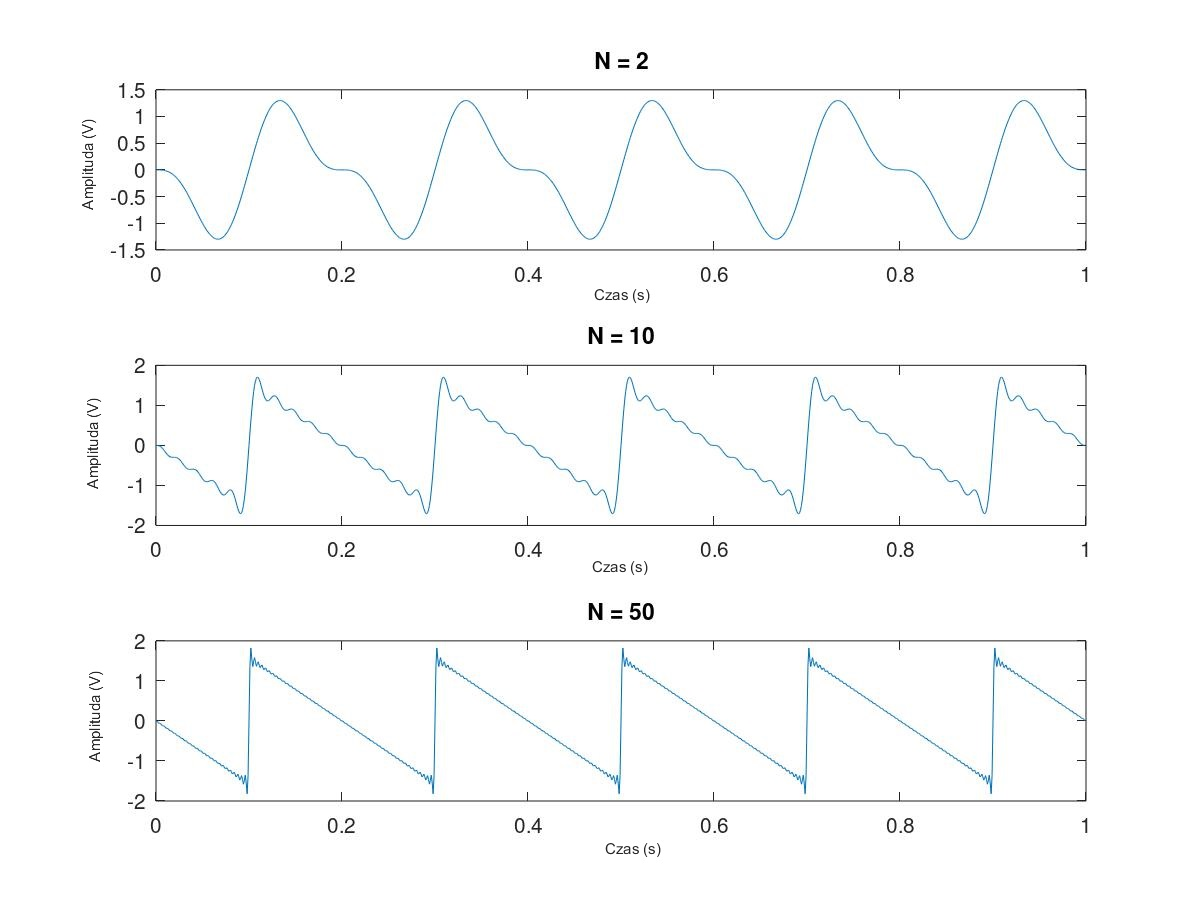
\includegraphics[width=12cm]{grafiki/add_sawtooth}
	\captionsetup{justification=centering}
	\caption{Generacja przebiegu piłokształtnego za pomocą syntezy addytywnej.}
	\label{rys:add_sawtooth}
\end{figure}

Na rysunku \ref{rys:add_sawtooth} przedstawiono wygenerowany przebieg piłokształtny, jako przykład addytywnej syntezy dźwięku w postaci harmonicznej. Na pierwszym z wykresów przedstawiono przebieg uzyskany z dwóch składowych harmonicznych, a na kolejnym z dziesięciu. Na ostatnim wykresie widać przebieg składający się z 50 SH, który jest dobrą aproksymacją idealnego przebiegu piłokształtnego. Sygnał został wygenerowany na podstawie wzoru (\ref{equ:addit_sawth}).

\subsection{Postać nieharmoniczna} \label{pos_nieharm}
Dobieranie składowych dźwięku w syntezie addytywnej nie musi zależeć od konkretnej częstotliwości podstawowej. Niektóre instrumenty wydają dźwięk składający się ze składowych harmonicznych oraz nieharmonicznych (czyli takich, które nie są całkowitą wielokrotnością pewnej częstotliwości $f_{0}$). Zsyntezowany dźwięk w takiej postaci można opisać wzorem:
\begin{equation} \label{equ:addit_time_nieharm}
y(t) = \sum_{k=1}^{K} a_{k}sin(2\pi f_{k}t + \phi_{k})  \\  
\end{equation}
\begin{tabular}{ l l l l}
	gdzie: 	&	$f_{k}$ & - &  częstotliwość składowej sygnału k,\\
\end{tabular} \\

Postać (\ref{equ:addit_time_nieharm}) można traktować jako uogólnioną formę wzoru (\ref{equ:addit_time_harm}). Dźwięk opisany powyższym wzorem jest generowany przez instrumenty takie jak dzwony lub perkusjonalia.

\subsection{Składowe zmienne w czasie}
%https://books.google.pl/books/about/The_Computer_Music_Tutorial.html?id=nZ-TetwzVcIC&printsec=frontcover&source=kp_read_button&redir_esc=y#v=onepage&q&f=false  , strona 140
Wzory matematyczne (\ref{equ:addit_time_harm}) i (\ref{equ:addit_time_nieharm}) pozwalają na uzyskanie jedynie stanu ustalonego zsyntezowanego brzmienia. Powtarzany jest jeden okres sygnału, co daje wrażenie słuchaczowi, iż barwa dźwięku jest bardzo prosta.

Składowe dźwięku mogą jednak zmieniać się w czasie \cite{add_time_varying}. Zmiany te mogą dotyczyć ich amplitudy, jak i częstotliwości.
Taką postać syntezy addytywnej zapisuje się:
\begin{equation} \label{equ:addit_time_zmienne}
y(t) = \sum_{k=1}^{K} a_{k}(t)sin(2\pi f_{k}(t)t + \phi_{k})  \\  
\end{equation}
\begin{tabular}{ l l l l}
	gdzie: & $a_{k}(t)$ &  - & zmienna w czasie amplituda składowej k, \\
	&	$f_{k}(t)$ & - &  zmienna w czasie częstotliwość składowej k, \\
\end{tabular} \\

Realizacja brzmienia na podstawie wzoru (\ref{equ:addit_time_zmienne}) może być rozumiana jako zmiana parametrów instrumentu w trakcie generowania przez niego dźwięku.

\subsection{Szum w syntezie addytywnej}
%https://ccrma.stanford.edu/~jos/sasp/S_N_Synthesis.html
Tworzenie dźwięku zsyntezowanego metodą addytywną za pomocą wzorów przedstawionych powyżej jest deterministyczne. Do takiego sygnału może zostać dodana część stochastyczna. Uzyskuje się to poprzez wykorzystanie zmiennego w czasie filtra FIR oraz białego szumu \cite{add_szum}.

\begin{equation} \label{equ:addit_szum}
B(\omega) = F(\omega)*e^{j\phi(\omega_{k})} \\  
\end{equation}
\begin{tabular}{ l l l l}
	gdzie: & $\phi(\omega_{k})$ &  - & faza losowa o rozkładzie równomiernym od -$\pi$ do $\pi$, \\
	& $F(\omega)$ &  - & obwiednia widmowa filtra FIR o zmiennych parametrach, \\
	&	$B(\omega)$ & - & zmienna w czasie częstotliwość składowej k, \\
\end{tabular} \\

Synteza części stochastycznej polega na przetwarzaniu białego szumu (bazującego na losowej fazie) przez filtr FIR. Takie działanie zostało zaprezentowane we wzorze (\ref{equ:addit_szum}). Następnie część stochastyczna zostaje przetransformowana do dziedziny czasu. Ostatnim krokiem jest zsumowanie ze sobą obu części.

Dodanie szumu do sygnału deterministycznego w syntezie addytywnej pozwala na uzyskanie dźwięków na przykład instrumentów dętych. Część stochastyczna sygnału sprawia wrażenie dmuchania w instrument.

% Mozna jeszcze to użyć:
%https://ccrma.stanford.edu/~jos/sasp/Sines_Noise_Analysis.html

\section{Metody implementacji syntezy addytywnej}
Istnieją różne metody implementacji addytywnej syntezy dźwięku \cite{add_imp_meth}. Oznacza to, iż sam dźwięk może zostać uzyskany różnymi sposobami. Popularne metody realizacji syntezy addytywnej to:
\begin{itemize}
	\item bank oscylatorów,
	\item synteza wavetable,
	\item synteza IFFT.
	% https://ieeexplore.ieee.org/document/4412805
\end{itemize}
W niniejszym podrozdziale przedstawiono ograniczenia syntezy addytywnej oraz wytłumaczono wymienione wyżej metody implementacji.

\subsection{Ograniczenia syntezy addytywnej} \label{addit_ograniczenia}
%https://en.wikipedia.org/wiki/Additive_synthesis#History
Synteza addytywna w instrumentach klawiszowych jest używana między innymi do generacji dźwięku organów, których barwa upraszczana jest zazwyczaj do kilku SH. W przypadku próby uzyskania dźwięku o większej ilości składowych harmonicznych, złożoność obliczeniowa metody wzrasta \cite{add_ograniczenia}.
%https://ccrma.stanford.edu/~jos/pasp/Additive_Synthesis.html
Przykładowo, dla uzyskania pojedynczego dźwięku pianina w jakości CD-Audio,
%https://en.wikipedia.org/wiki/Compact_Disc_Digital_Audio
wymagane byłoby obliczenie około 400 fal sinusoidalnych na każdą próbkę zsyntezowanego dźwięku. Oznacza to, iż dla polifonicznej klawiatury takiego pianina mogłyby być to tysiące składowych przypadających na jedną próbkę. Obecne ograniczenia sprzętowe nie umożliwiają realizacji w czasie rzeczywistym tak skomplikowanych brzmień za pomocą syntezy addytywnej, z uwagi na zbyt dużą złożoność obliczeniową. Powstrzymują one szybki rozwój tej metody.

\subsection{Bank oscylatorów}
%analogowe hammondy i zwykłe, ale ze są wolne
Synteza przez bank oscylatorów jest najstarszą metodą implementacji addytywnej syntezy dźwięku. Opiera się ona bezpośrednio na równaniu (\ref{equ:addit_time_harm}).
Ta metoda implementacji realizowana była nawet na instrumentach analogowych. Instrumenty takie jak organy Hammonda posiadały kilka dyskowych wirników, które były nacięte w wielu miejscach na ich powierzchni. Obracające wirniki generowały prąd elektryczny o charakterystyce zawierającej pewne składowe harmoniczne tonu podstawowego.
\begin{figure}[H]
	\centering
	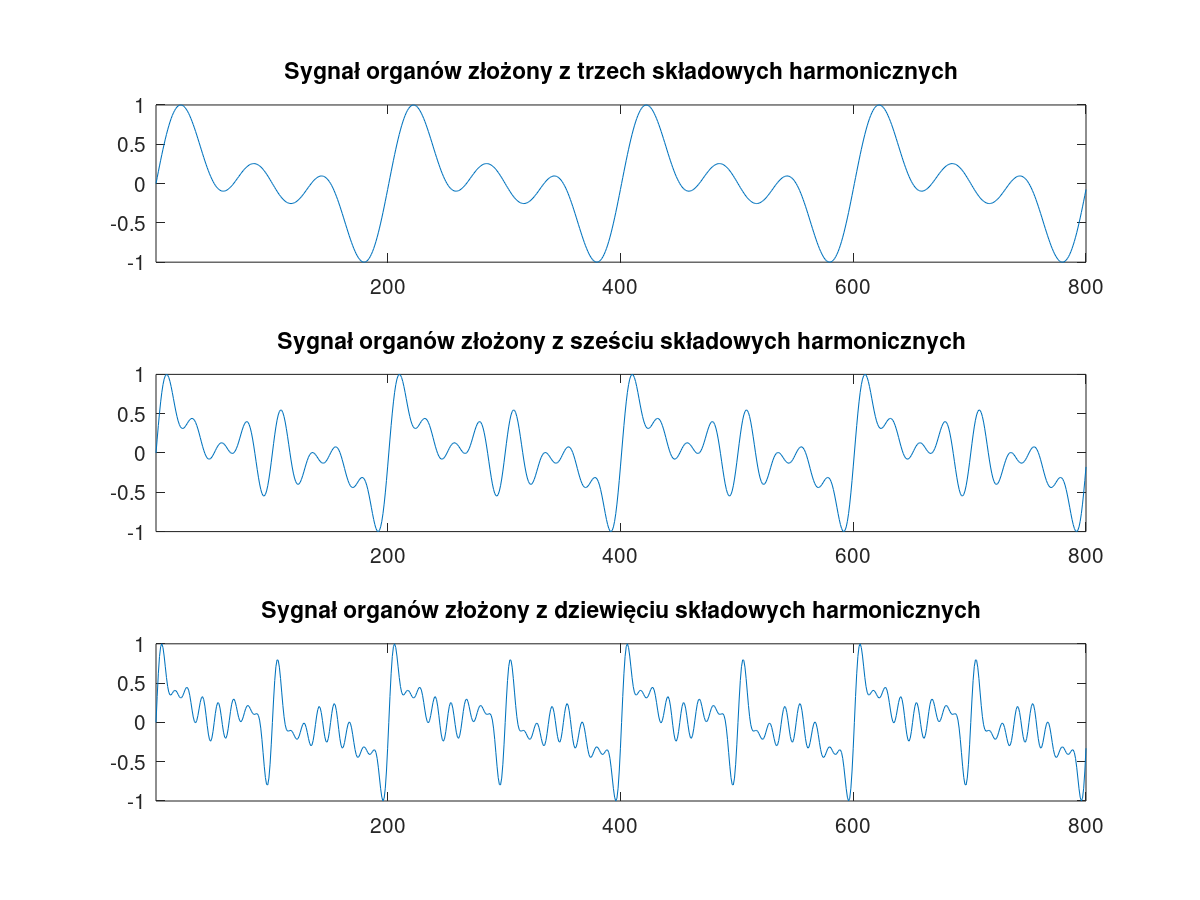
\includegraphics[width=15cm]{grafiki/add_hammond_matlab}
	\captionsetup{justification=centering}
	\caption{Barwa dźwięku organów Hammonda dla różnych ilości składowych harmonicznych.}
	\label{rys:add_hammond_matlab}
\end{figure}

Implementacja na procesorach DSP, odpowiadająca dyskowym wirnikom, opiera się na realizowaniu wielu funkcji sin() o różnych częstotliwościach i amplitudach. Każda taka funkcja generuje jedną składową harmoniczną syntezowanego dźwięku. Wszystkie razem traktowane są jako bank oscylatorów. Problem realizacji skomplikowanego brzmienia takim sposobem został przedstawiony w punkcie \ref{addit_ograniczenia}.

Na rysunku \ref{rys:add_hammond_matlab} przedstawiono wygenerowaną barwę organów Hammonda dla trzech różnych ustawień amplitud składowych harmonicznych. Najbardziej zauważalna różnica występuje między pierwszym i ostatnim wykresem. Dodanie dziewięciu SH bardzo zmienia charakter zsyntezowanego brzmienia w stosunku do sumowania jedynie trzech z nich.


\subsection{Synteza wavetable} \label{add_wavetable}
%opisac tą która została zaimplementowana
Synteza wavetable (nazywana również syntezą tablicową) polega na zapisaniu jednego okresu fali dźwiękowej do tablicy typu lookup zdefiniowanej w programie komputerowym \cite{add_wavetab_synt}. W każdej kolejnej chwili czasu działania programu, odczytywany jest odpowiedni element tablicy. Okres fali zapisanej w tablicy powinien zawierać nadmierną liczbę próbek (ang. over-sampled), aby móc odczytać go dla fal o niskich częstotliwościach. Niewystarczające spróbkowanie może doprowadzić do znacznych skoków wartości próbek generowanego dźwięku za pomocą metody wavetable.

W syntezie addytywnej użycie takiej metody implementacji może znacznie przyspieszyć generowanie kolejnych próbek składowych sygnału. Do tablicy zapisuje się jeden przebieg sinusoidalny. Odczyt jednego indeksu zabiera mniej czasu pracy procesora niż wygenerowanie próbki z funkcji sin(). Działanie takiej metody jest podobne do banku oscylatorów, ze względu na to, iż również realizowana jest w dziedzinie czasu. Znaczna różnica jest taka, że tablicę w syntezie wavetable można traktować jako jeden oscylator, z którego należy jedynie odczytać wartości tj. znaleźć odpowiedni indeks tablicy. Nie trzeba w każdej chwili czasu obliczać na nowo próbki dla każdej składowej dźwięku.
%https://en.wikipedia.org/wiki/Lookup_table

\subsection{Synteza IFFT}
%Rysunki z matlaba
W 1990 roku P. Depalle oraz X. Rodet \cite{add_ifft_orig} przedstawili przełomową metodę implementacji syntezy addytywnej. W ich podejściu obliczanie składowych dźwięku nie opiera się na zestawie oscylatorów, lecz na algorytmie IFFT (ang. Inverse Fast Fourier Transform) stosowanym dla krótkiego okna widma (STS, ang. short term spectrum) \cite{add_ifft_method}. Wyniki ich pracy dowiodły, iż udało im się zmniejszyć koszt obliczeń syntezy addytywnej piętnastokrotnie, w stosunku do metody banku oscylatorów (w ich indywidualnym przypadku, gdzie obliczali 9 istotnych punktów widma w 256 próbkowym STS).

Konstrukcja pojedynczej ramki STS została przedstawiona poniżej. Niech $f_{j}$, $a_{j}$ oraz $\phi_{j}$ będą średnimi wartościami częstotliwości, amplitudy i fazy ramki czasowej pożądanego sygnału $w[n]$. $W$ niech będzie Transformatą Fouriera okna sygnału $w[n]$. Dodanie pojedynczej składowej do STS może być zapisana zależnością:

\begin{equation} \label{equ:addit_IFFT}
S[k] = a_{j}e^{i\phi_{j}}W[f_{j} - k] \\  
\end{equation}
\begin{tabular}{ l l l l}
	gdzie: & $S[k]$ &  - & STS syntezowanego sygnału, \\
	& $W[f_{j} - k]$ &  - & przesunięte widmo sygnału $w[n]$, \\
	& $a_{j}e^{i\phi_{j}}$ & - & zespolona amplituda. \\
\end{tabular} \\

Wzór (\ref{equ:addit_IFFT}) oznacza, iż okno widmowe $W[f_{j} - k]$ zostanie wycentrowane na częstotliwości $f_{j}$ oraz przemnożone przez amplitudę $a_{j}e^{i\phi_{j}}$. Po takim działaniu w dziedzinie częstotliwości, okno STS poddane jest algorytmowi IFFT, którego rezultatem jest okno czasowe $s[n]$. Kolejne okna czasowe zakładkowane są metodą overlap-add. Końcowo otrzymuje się pełen sygnał zsyntezowanego dźwięku za pomocą syntezy IFFT.

Dodanie szumu do sygnału jest również bardziej efektywne obliczeniowo w przypadku stosowania opisywanej metody implementacji syntezy addytywnej. Szum biały może zostać dodany już na etapie tworzenia STS, a następnie poddany algorytmowi IFFT. Ostatecznie uzyskiwane jest okno sygnału zawierającego część deterministyczną, jak i stochastyczną.

\section{Interfejs użytkownika}
W autorskim projekcie, w ramach realizacji instrumentu klawiszowego z syntezą addytywną, zaimplementowano program generujący dźwięk organów Hammonda. 
%https://www.soundonsound.com/techniques/synthesizing-tonewheel-organs-part-1
Laurens Hammond, twórca tychże organów, zaprojektował je tak, aby użytkownik miał możliwość doboru amplitudy dziewięciu składowych harmonicznych generowanego dźwięku \cite{add_hammond_soundonsound}. Każda z nich była regulowana suwakiem na 8 możliwych poziomów. Suwaki oznaczały kolejne wartości amplitudy pierwszej, drugiej, trzeciej, czwartej, szóstej, ósmej, dziesiątej, dwunastej oraz szesnastej składowej harmonicznej dźwięku. Przykładowe różnice w generowanej barwie organów przedstawione zostały na rysunku \ref{rys:add_hammond_matlab}.
\begin{figure}[H]
	\centering
	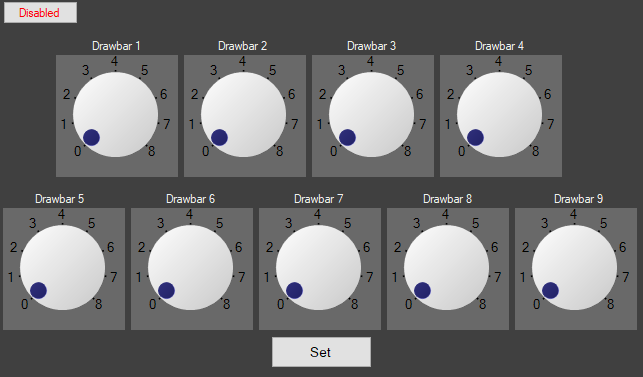
\includegraphics[width=15cm]{grafiki/add_interface}
	\captionsetup{justification=centering}
	\caption{Interfejs użytkownika dla syntezy addytywnej.}
	\label{rys:add_interface}
\end{figure}

Interfejs użytkownika opiera się na oryginalnym instrumencie Laurensa Hammonda. Umożliwia on użytkownikowi regulację dziewięciu SH za pomocą gałek przedstawionych na rysunku \ref{rys:add_interface}. Można zauważyć, iż gałki posiadają również 8 poziomów wartości, które odpowiadają wartościom amplitud składowych harmonicznych. Po ustawieniu pożądanej barwy, użytkownik musi kliknąć w panelu przycisk "Set", aby parametry syntezy addytywnej zostały wysłane do procesora DSP.

Gałki w panelu zostały zrealizowane za pomocą obiektów klasy KnobControl. Naciśnięcie przycisku "Set" wywołuje funkcję, która odczytuje wartość elementu panelu syntezy addytywnej w formie tablicy bajtów. Następnie wysyła odpowiedni identyfikator gałki do procesora DSP, a po nim jej wartość odczytaną z tablicy.

\section{Realizacja organów na procesorze DSP}
Pierwszą próbą implementacji organów Hammonda w autorskim programie na procesor DSP, było wykorzystanie metody banku oscylatorów. Rezultaty były jednak niezadowalające. Wywołanie funkcji sin() dziwięciokrotnie dla jednej próbki sygnału, oznaczało, iż w podejściu polifonicznym mogła ona zostać wywołana nawet dziewiędziesiąt razy (przykład dla naciśniętych dziesięciu klawiszy na klawiaturze MIDI).
Pomimo zastosowanego mechanizmu zakładkowania, w generowanym dźwięku pojawiały się niepożądane artefakty świadczące o zbyt dużej złożoności obliczeniowej zaimplementowanego algorytmu. Należało zmienić podejście do implementacji syntezy addytywnej.

Ostatecznie w autorskim programie komputerowym na procesor DSP wykorzystano metodę implementacji z użyciem tablicy wavetable, która została omówiona w punkcie \ref{add_wavetable}. W niniejszym podrozdziale został przedstawiony sposób realizacji programu umożliwiającego syntezę dźwięku organów Hammonda oraz rezultaty takiej syntezy na układzie TMS320C6727.

\subsection{Opis implementacji}
Zdefiniowana tablica lookup o nazwie sinLut[.] zawiera jeden okres fali sinusoidalnej. Wypełniona zostaje na etapie inicjalizacji programu na procesorze DSP. Każdy element tablicy zostaje odczytany za pomocą funkcji mySin(), która jako argumenty przyjmuje częstotliwość pożądanej fali sinusoidalnej oraz jej przesunięcie w fazie.
\begin{equation} \label{equ:addit_sinLut}
\text{samp} = \text{sinLut}[(kf\frac{N}{F_s})\mod{N}] \\  
\end{equation}
\begin{tabular}{ l l l l}
	gdzie: & \text{samp} &  - & wartość próbki odczytywanej z tablicy sinLut[.], \\
	& $k$ &  - & licznik odczytu odpowiedniej próbki z tablicy sinLut[.], \\
	& $f$ & - & częstotliwość sinusoidy, \\
	& $N$ & - & długość tablicy sinLut[.], \\
	& $F_s$ & - & częstotliwość próbkowania DAC. \\
\end{tabular} \\

Funkcja mySin() zwraca element z tablicy na podstawie wzoru (\ref{equ:addit_sinLut}). Do wygenerowania jednej próbki organów Hammonda sumowane jest 9 tak odczytanych wartości sinLut[.] (odpowiadających składowym harmonicznym). Każda próbka zsyntezowanego dźwięku ulega wymnożeniu z obecną wartością amplitudy ADSR. Opisana czynność wykonywana jest tyle razy, ile elementów posiada jeden blok generowanego sygnału.

Procesor DSP otrzymuje nastawy gałek syntezy addytywnej z interfejsu użytkownika w obsłudze przerwania UART. Parametry te są zapisywane do tablicy add\_knobAmp[.]. Następnie są używane do syntezy dźwięku organów.

\subsection{Wyniki}
Wykorzystana metoda implementacji za pomocą tablicy wavetable umożliwiła naciśnięcie nawet kilkunastu klawiszy instrumentu, bez pojawienia się niepożądanych artefaktów w dźwięku. Zmiany amplitud poszczególnych składowych harmonicznych wpływają na generowane w brzmienie w bardzo wyraźny sposób.

\begin{figure}[H]
	\centering
	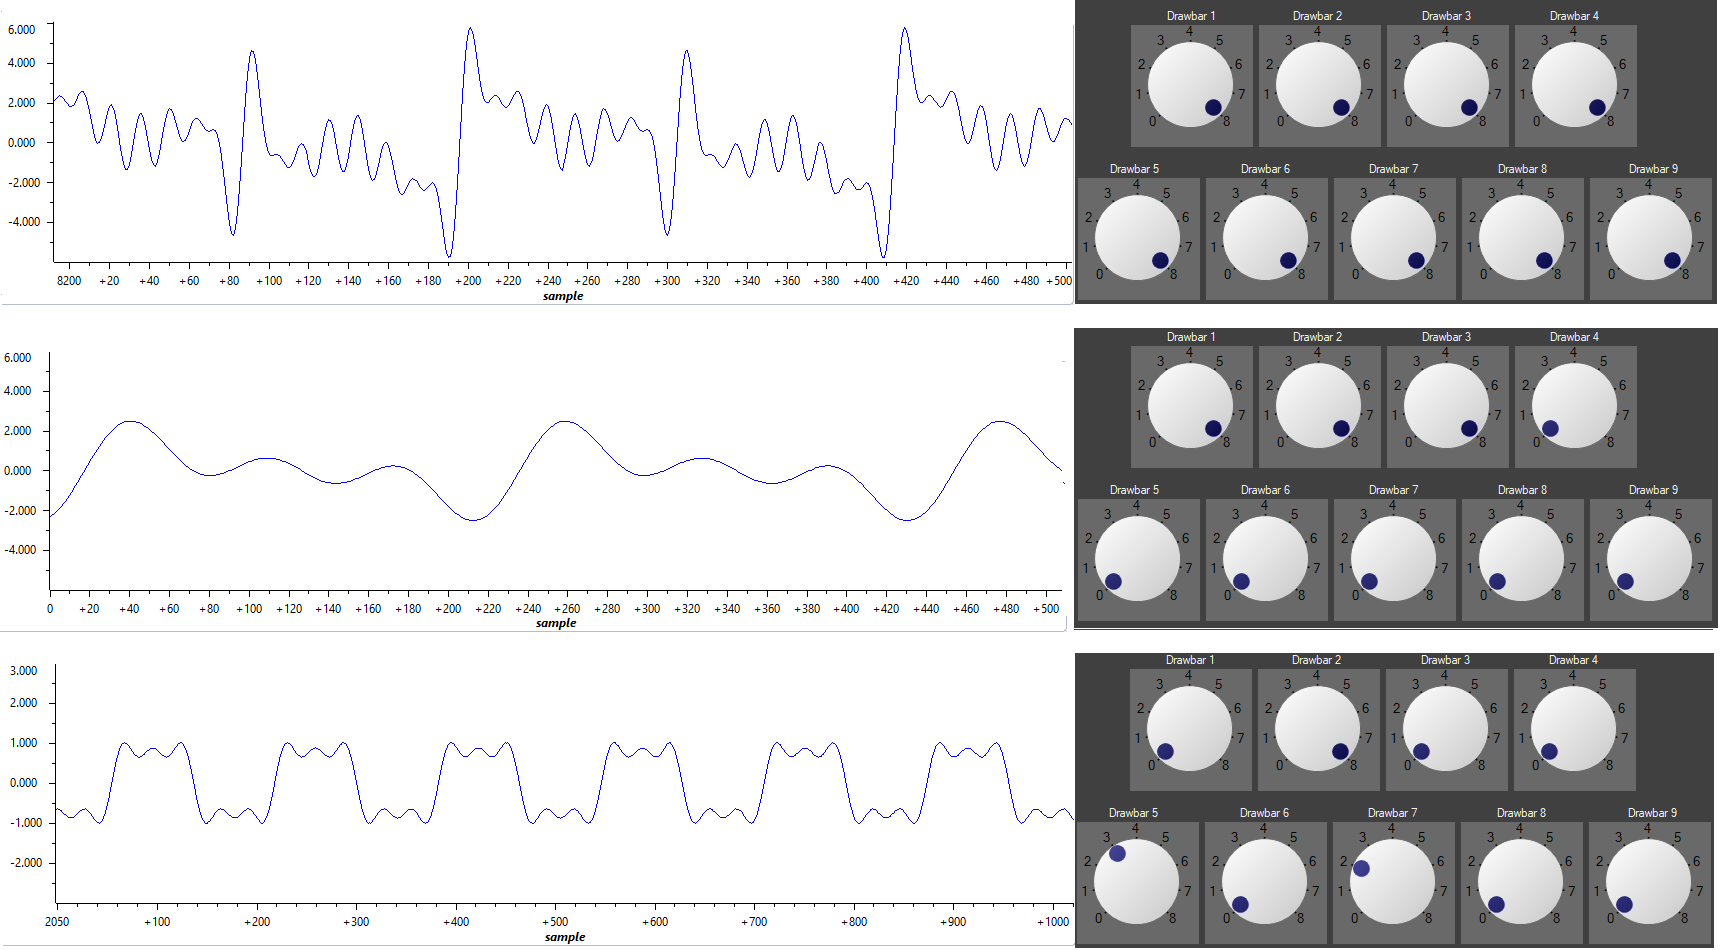
\includegraphics[width=15cm]{grafiki/add_hammond_dsp}
	\captionsetup{justification=centering}
	\caption{Wizualizacja sygnału dźwiękowego organów Hammonda z procesora DSP dla różnych nastaw gałek.}
	\label{rys:add_hammond_dsp}
\end{figure}

Na rysunku \ref{rys:add_hammond_dsp} przedstawiono wizualizację sygnału organów dla różnych ustawień gałek w interfejsie użytkownika. Na wykresie pierwszym od góry wszystkie SH mają maksymalną amplitudę (konfiguracja "8888 88888"). Tak wygenerowany dźwięk bardzo przypomina brzmienie katedralnych organów piszczałkowych. Na kolejnym wykresie przedstawiono sygnał utworzony przy konfiguracji gałek na wartościach "8880 00000". Brzmienie dźwięku przy takim ustawieniu gałek jest dużo bardziej delikatne niż w pierwszej konfiguracji. Na najniższym wykresie ustawienie amplitud to "0800 30200". Można zauważyć, iż wizualnie bardzo przypomina przebieg prostokątny. Brzmienie tak wygenerowanego dźwięku również jest zbliżone do dźwięku przebiegu prostokątnego.

Przedstawione barwy organów mogą brzmieć jeszcze lepiej po dodaniu takich efektów jak Chorus lub Vibrato. Do uzyskania pełni brzmienia takich organów, często również stosuje się efekt pogłosu (ang. reverb).